\documentclass[a4paper,norsk]{article}
\usepackage[utf8]{inputenc}
\usepackage[T1]{fontenc,url}
\usepackage{babel,textcomp}
\usepackage{graphicx}
\usepackage{amsmath}
\usepackage{cleveref}
\usepackage[cmyk]{xcolor}
\usepackage{listings}
\graphicspath{ {./images/} }
\lstset {language=C++,    
backgroundcolor=\color{yellow!20},    
commentstyle=\color{green},    
%keywordstyle=\color{blue},    
basicstyle=\footnotesize}
\urlstyle{sf}
\title{Oblig 2 Matte 3}
\date{\today}
\author{Adam Aske}
\newpage
\begin{document}
\maketitle
\tableofcontents
\newpage
 \section{Github}
Link til min branch : https://github.com/Hedmark-University-College-SPIM/3Dprog22/tree/AdamA
\section{Oppgave 3.4.6}
Oppgave 3.4.6
Valgte punkter: (-6, 10), ( -5.9, 6.6), (-3, 4.8), (-3.1, 1.60), (0.1, 0.5), (2.6, 1.1), (3.8, 4.3), (6.7, 5.2)\newline
Wolfram Aplha er brukt til matrise multiplikasjonene. \newline
y = Ax + e \newline
\begin{equation*} 
\begin{bmatrix}10 \\ 6.6\\4.8\\1.6\\0.5\\1.1\\4.3\\5.2\end{bmatrix}
=\begin{bmatrix}36 & -6 & 1 \\ 43.8 & -5.9 & 1 \\9 & -3 & 1 \\ 9.6 & -3.1 & 1 \\0 & 0.1 & 1 \\6.7& 2.6 & 1 \\14.4 & 3.8 & 1 \\ 44.9 & 6.7 & 1\end{bmatrix}\begin{bmatrix}a\\b\end{bmatrix}
+ \begin{bmatrix} e_1 \\ e_2 \\ e_3 \\ e_4 \\ e_5 \\ e_6 \\ e_7\end{bmatrix}
\end{equation*}

\begin{equation*}
B = A^{T} * A = \begin{bmatrix}36 & 34.8 & 9 & 9.6 & 0 & 6.7&14.4&44.9\\ -6 & -5.9 &-3&-3.1&0.1&2.6&3.8&6.7\\1 & 1 & 1 & 1& 1 & 1 & 1 & 1\end{bmatrix}
\begin{bmatrix}36 & -6 & 1 \\ 43.8 & -5.9 & 1 \\9 & -3 & 1 \\ 9.6 & -3.1 & 1 \\0 & 0.1 & 1 \\6.7& 2.6 & 1 \\14.4 & 3.8 & 1 \\ 44.9 & 6.7 & 1\end{bmatrix}
=\begin{bmatrix}4948.5 & -97.07 & 155.4 \\ -105.11 & 158.6 & -4.8 \\ 155.4 & -3.6 & 8\end{bmatrix}
\end{equation*} 

\begin{equation*}
C = A^{T} * y = \begin{bmatrix}36 & -6 & 1 \\ 43.8 & -5.9 & 1 \\9 & -3 & 1 \\ 9.6 & -3.1 & 1 \\0 & 0.1 & 1 \\6.7& 2.6 & 1 \\14.4 & 3.8 & 1 \\ 44.9 & 6.7 & 1 \end{bmatrix}
\begin{bmatrix}10 \\ 6.6\\4.8\\1.6\\0.5\\1.1\\4.3\\5.2\end{bmatrix}
=\begin{bmatrix} 951 \\ -64.2 \\ 34.1 \end{bmatrix}
\end{equation*}

\begin{equation*}
B^{-1} = \begin{bmatrix} 0.0005  & 0 & -0.01\\ 0 & 0.006 & 0.003 \\ -0.01 & 0.001 & 0.32 \end{bmatrix}
\end{equation*}

\begin{equation*}
x = B^{-1} * c = \begin{bmatrix} 00.0005  & 0 & -0.01\\ 0 & 0.006 & 0.003 \\ -0.01 & 0.001 & 0.32  \end{bmatrix}\begin{bmatrix} 951 \\ -64.2 \\ 34.1\end{bmatrix}
= \begin{bmatrix}0.145  \\ -0.268 & 1.309 \end{bmatrix}
\end{equation*}
$y = 0.145x^{2}-0.268x+1.309$
\section{Beregne punkter og lagre i array}
Funksjonen tar inn x som verdi og bruker funksjonen fra utergningen og returnerer y verdien punktet skal ha.
\begin{lstlisting}[language=C++, caption={trianglesurface.h}]
static float func2(float x) {
       return 0.174 * x + 1, 743;
   }
\end{lstlisting}
\section{3.4.6 Visualisering}
VisualPoint klassen tar inn en vector av Vertex'er, vertexene blir vist som hvite brikker på skjermen. MMap får en QuadraticPolynomial som tar inn 6.9, 1.3 og 3.2 fra minste kvadtraters metode, og blir vist som en grønn kurve på skjermen.
De stemmer ikke med hverandre, noe er feil med utregningen.
\begin{lstlisting}[language=C++, caption={renderwindow.cpp}]
mMap.insert(std::pair<std::string, VisualObject*>{"QuadtraticPolynomial", 
new QuadtraticPolynomial(0.145f, -0.268f, 1.3f, 0.1f)});
    std::vector<Vertex> points;
    points.push_back(Vertex{ -6, 10, 0 });
    points.push_back(Vertex{ -5.9, 6.6, 0 });
    points.push_back(Vertex{ -3, 4.8, 0 });
    points.push_back(Vertex{ -3.1, 1.6, 0 });
    points.push_back(Vertex{ 0.1, 0.5, 0 });
    points.push_back(Vertex{ 2.6, 1.1, 0 });
    points.push_back(Vertex{ 3.8, 4.3, 0 });
    points.push_back(Vertex{ 6.7, 5.2, 0 });

    for (auto i = 0; i < points.size(); i++) {
        mMap.insert(std::pair<std::string, VisualObject*>
{ std::to_string(i) , new VisualPoint(points)});
    }
\end{lstlisting}
Den ser noe forvrengt ut, men det skyldes kamera sin rotasjon.
\centering
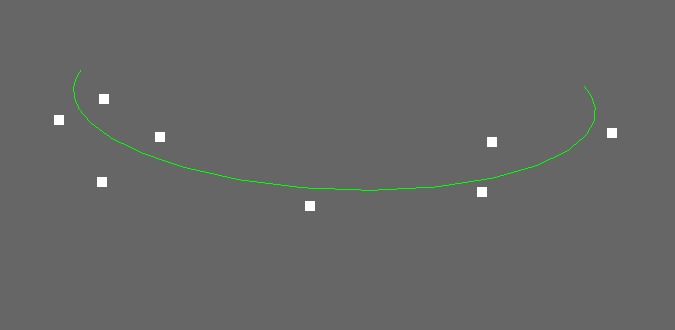
\includegraphics[width=\textwidth]{MatteOblig2Minstekvadratersmetode}

\section{Oppgave 4.6.7}
Punkter: ( 0.9, 0.6), ( 2.2, 2.6), (4.5, -1), (5.9, 1.6) 
\newline
$f(x) = ax^{3} + bx^{2} + cx + d$\newline
$0.6 = a*0.6^{3} + b*0.6^{2} + c*0.6 + d$\newline
$2.6 = a*2.6^{3} + b*2.6^{2} + c*2.6 + d$\newline
$-1 = -a*1^{3} - b*1^{2} - c*1 + d$\newline
$1.6 = a*1.6^{3} + b*1.6^{2} + c*1.6 + d$\newline
\begin{equation*}
A = \begin{bmatrix} 0.729  & 0.81 & 0.9 & 1 \\ 10.648 & 4.84 & 2.2 & 1 \\ 
91.125 & 20.25 & 4.5 & 1 \\  205.379 & 34.81  & 5.9 & 1\end{bmatrix} B = \begin{bmatrix} 0.6 \\ 2.6 \\ -1 \\ 1.6\end{bmatrix}\end{equation*}
\newline
\begin{equation*}
A^{-1} = \begin{bmatrix} -0.04  & 0.09 & -0.09 & -0.4 \\ 0.5 & -1.02 & 0.77 & -0.29 \\ 
-2.11 & 3.25 & -1.7 & 0.6 \\  2.5 & -2.15  & 1 & -0.34 \end{bmatrix}
\end{equation*}
\newline
$x = A^{-1}*B = $
\begin{equation*}
\begin{bmatrix}  -0.04  & 0.09 & -0.09 & -0.4 \\ 0.5 & -1.02 & 0.77 & -0.29 \\ 
-2.11 & 3.25 & -1.7 & 0.6 \\  2.5 & -2.15  & 1 & -0.34  \end{bmatrix} \begin{bmatrix}  0.6 \\ 2.6 \\ -1 \\ 1.6\end{bmatrix}
= \begin{bmatrix} -0.34 \\ - 3.586 \\ 9.844 \\  -5.634 \end{bmatrix}
\newline
f(x) = -0.34x^{3} - 3.586x^{2}+9.844x - 5.634
\end{equation*}
\section{4.6.7 Visualisering}
VisualPoint klassen tar inn en vector av Vertex'er, vertexene blir vist som hvite brikker på skjermen. MMap får en QuadraticPolynomial som tar inn 6.9, 1.3 og 3.2 fra minste kvadtraters metode, og blir vist som en grønn kurve på skjermen.
De stemmer ikke med hverandre, noe er feil med utregningen.
\begin{lstlisting}[language=C++, caption={renderwindow.cpp}]
//Matte oblig 2 4.6.7
    mMap.insert(std::pair<std::string, VisualObject*>{"CubicPolynomial", new CubicPolynomial(-0.34, -3.586, 9.844, -5.634,0.1f)});
    std::vector<Vertex> points2;
    points2.push_back(Vertex{ 0.9f, 0.6f, 0 });
    points2.push_back(Vertex{ 2.2f, 2.6f, 0 });
    points2.push_back(Vertex{ 4.5f, -1.f, 0 });
    points2.push_back(Vertex{ 5.9f, 1.6, 0 });
    
    for (auto i = 0; i < points2.size(); i++) {
        mMap.insert(std::pair<std::string, VisualObject*>{ std::to_string(i*10), new VisualPoint(points2)});
    }
\end{lstlisting}
\begin{lstlisting}[language=C++, caption={cubicpolynomial.cpp}]
CubicPolynomial::CubicPolynomial(double a, double b, double c, double d, float dx)
{
   
    for (auto x = -10.f; x <= 10; x += 0.1)
    {
        auto y = p(a, b, c, d, x);
        mVertices.push_back(Vertex(x, y, 0, 0, 1, 0));
    }
    mMatrix.setToIdentity();

}

double CubicPolynomial::p(double a, double b, double c, double d, double x)
{
    return a * x * x * x + b * x * x + c * x + d;

}
\end{lstlisting}
Resultatet ser ikke riktig ut i mine øyne, men har omregnet matrisene flere gangene. 
\centering
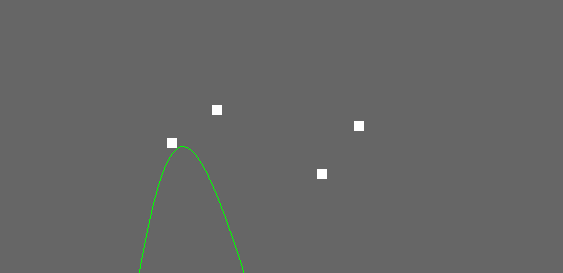
\includegraphics[width=\textwidth]{MatteOblig2Kubiskinterpolasjon}

\section{Oppgave 4.11.6}
\end{document}